\documentclass[conference, spanish]{IEEEtran}

\ifCLASSINFOpdf
   \usepackage[pdftex]{graphicx}
  % declare the path(s) where your graphic files are
   \graphicspath{{../pdf/}{../jpeg/}}
  % and their extensions so you won't have to specify these with
  % every instance of \includegraphics
   \DeclareGraphicsExtensions{.pdf,.jpeg,.png}
\else
  % or other class option (dvipsone, dvipdf, if not using dvips). graphicx
  % will default to the driver specified in the system graphics.cfg if no
  % driver is specified.
  \usepackage[dvips]{graphicx}
  % declare the path(s) where your graphic files are
  \graphicspath{{../eps/}}
  % and their extensions so you won't have to specify these with
  % every instance of \includegraphics
  \DeclareGraphicsExtensions{.eps}
\fi


\usepackage[utf8x]{inputenc}
\usepackage[T1]{fontenc}
\usepackage{booktabs}
\usepackage{subfigure}
\usepackage[colorlinks=true,linkcolor=black,urlcolor=black,citecolor=black, urlcolor=black, filecolor=black bookmarks=false]{hyperref}

\begin{document}

\pagestyle{empty}  

\title{Análisis de regresión para el cálculo de biomasa en el departamento de Nariño (Colombia) utilizando imágenes satelitales Landsat}

\author{\IEEEauthorblockN{GIEE}
\IEEEauthorblockA{Universidad de Nariño\\
San Juan de Pasto, Colombia\\
Email: }
\and
\IEEEauthorblockN{GIIWW}
\IEEEauthorblockA{Universidad de Nariño\\
San Juan de Pasto, Colombia\\
Email: }
}

\maketitle

\begin{abstract}

En este artículo se describen los componentes básicos de la investigación aplicada que tiene como objetivo construir un primer mapa del potencial de biomasa en el departamento de Nariño (Colombia) a partir de imágenes satelitales Landsat de libre acceso. Se analizan las diferentes bandas de las imágenes satelitales disponibles y su relación con bases de datos previas de biomasa aplicando diferentes técnicas de regresión y obteniendo un modelo para la generación de mapas actualizados en el departamento de Nariño.

\end{abstract}


\begin{IEEEkeywords}
biomass, regression models 
\end{IEEEkeywords}

\thispagestyle{empty} 

\IEEEpeerreviewmaketitle


\section{Introducción}

\IEEEPARstart 
En las últimas décadas la investigación en fuentes alternativas de energía ha recibido particular atención y ha pasado de tener un alto interés en los círculos académicos a convertirse en un punto prioritario en la agenda de gobiernos y organizaciones a nivel mundial.  La dependencia en combustibles fósiles y acuerdos internacionales como el protocolo de Kyoto han impulsado aún más el interés alrededor del tema.  En particular, la implementación de soluciones como páneles fotovoltáicos, parques eólicos y plantas de biomasa han atraido gran atención en especial en zonas con baja o nula cobertura.

En Colombia, según estudios del Ministerio de Minas y Energía, en el departamento de Nariño hay 15 municipios con cobertura eléctrica inferior al 80\% \cite{ministerio_de_minas_y_energia_plan_2008}. Como nueva estratégia para enfrentar esta problemática se ha propuesto el estudio y análisis de fuentes alternativas de energía en la zona. Uno de los principales objetivos es la medición y estimación de potenciales energéticos para identificar las zonas más viables en la región donde efectuar pruebas piloto y estudios de factibilidad. 

Sin embargo, uno de los principales retos para la ubicación de dichas zonas es la ausencia de bases de datos actualizadas así como series de tiempo históricas que apoyen el proceso de toma de decisiones.  Igualmente, restricciones de tiempo y costos impiden el despliegue de trabajo de campo para la recolección de información.  En el caso del análisis del potencial biomásico, estas restricciones se acentuan debido a la toma manual de muestras, extensión del área de estudio, análisis de laboratorio, dificultad del terreno e, incluso, presencia de grupos armados en la zona. 

En este sentido, diversas investigaciones han demostrado la utilidad del uso de imágenes satelitales para la generación de modelos que permitan calcular la cantidad de biomasa presente en un determinado lugar. Desde hace más de 30 años, se cuenta con acceso al repositorio de imágenes satelitales Landsat \cite{landsat} de manera libre y gratuita.  Bajo el debido tratamiento, estas imágenes pueden ser usadas para calcular valores nominales de biomasa a partir de modelos de regresión y trabajo de campo.  Sin embargo, dadas las dificultades para realizar dicho trabajo de campo, este estudio propone utilizar imágenes provistas por investigaciones anteriores.   \cite{baccini2008afirst} y \cite{baccini_estimated_2012} proporcionan bases de datos de los índices de biomasa a nivel pan-tropical entre los años 2000 y 2003.  Al igual que el conjunto de imágenes Landsat, las imágenes georreferenciadas para cada uno de los países analizados son de libre acceso y se encuentran disponibles en \cite{WHRC}.

Esta investigación presenta la metodología propuesta para la generación de un modelo de predicción de biomasa, basado en modelos de regresión e imágenes satelitales de libre acceso, y su extrapolación al resto del área de estudio.

El area de estudio de esta investigación fue el departamento de Nariño, el cual esta ubicado en el extremo Suroccidental de Colombia (en la frontera con Ecuador) con una extensión aproximada de 33.268 km, una población de 1,702 millones (según
el censo de 2013) y ubicada entre coordenadas 00° 31' 08'' y 02° 41' 08'' Norte y 76° 51' 19'' y 79° 01' 34'' Oeste (figura  \ref{fig:locationNarino}).

\begin{figure}
  \centering
  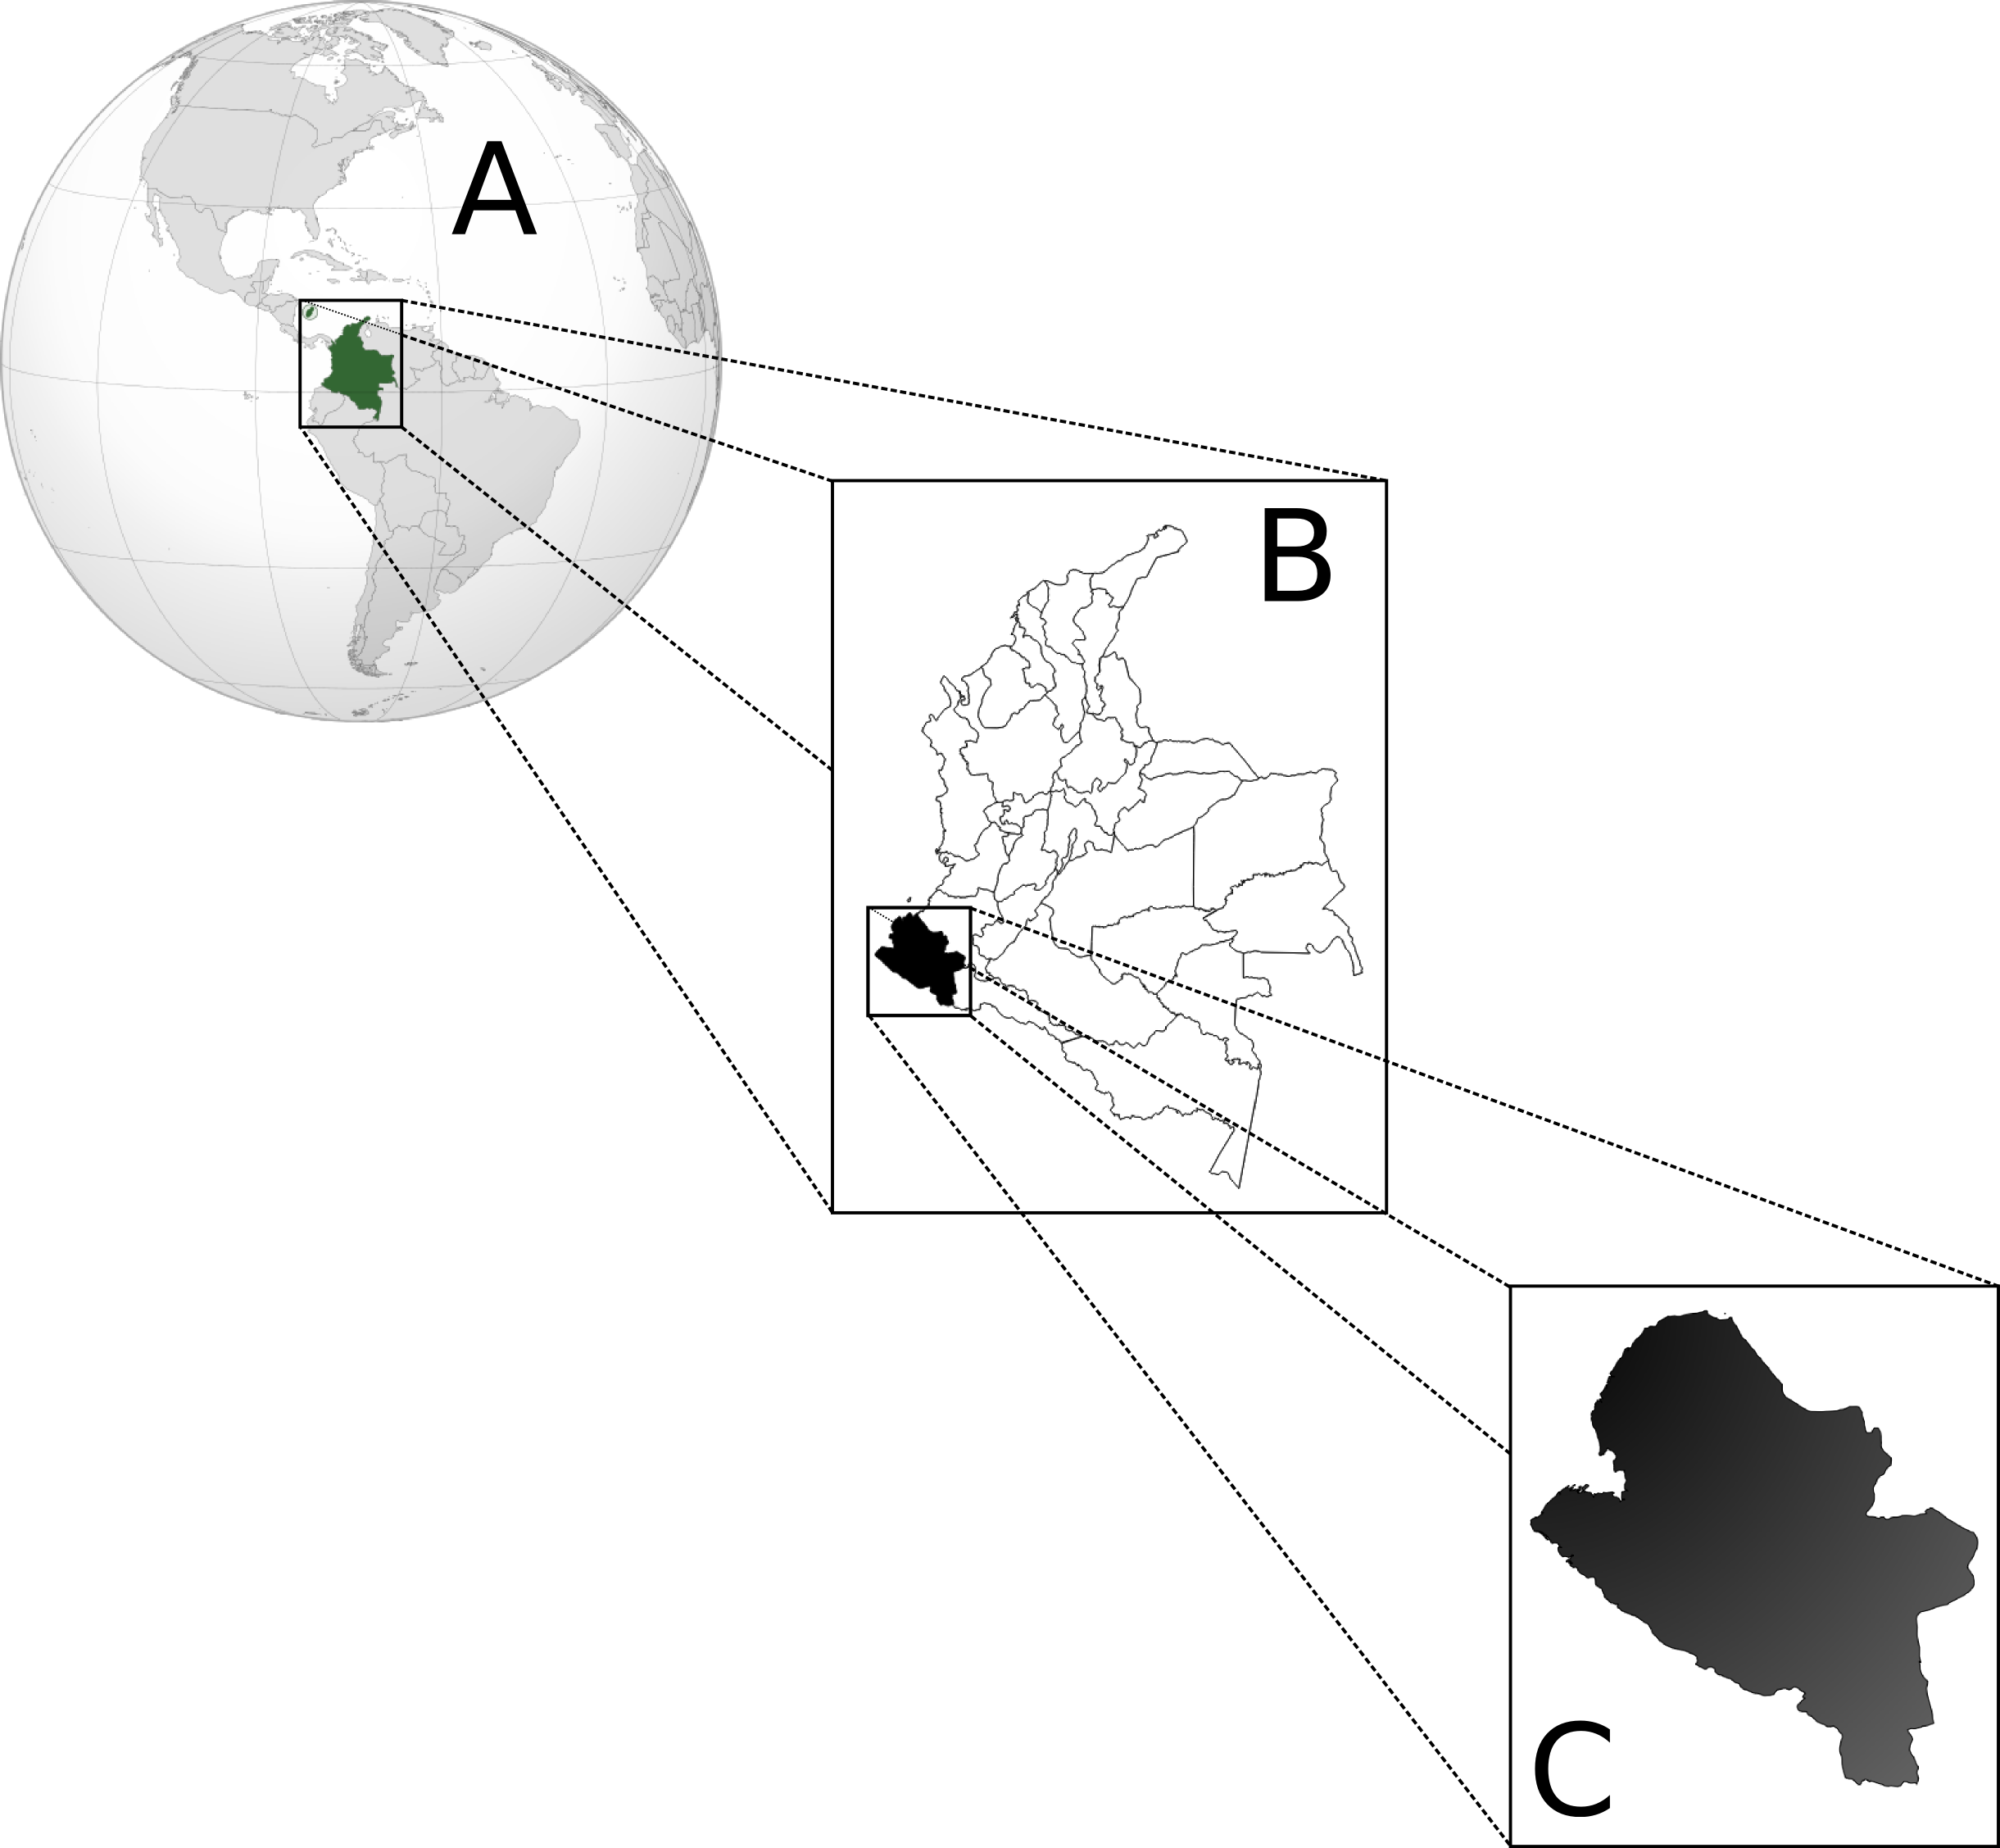
\includegraphics[width = 8cm]{locationNarino.png}
  \caption{Localización area de estudio}
  \label{fig:locationNarino}
\end{figure}
\section{Trabajos relacionados}

Diferentes estudios han explorado la construcción de mapas eólicos a partir
 de muestras tomadas en terreno.
 Por ejemplo, \cite{haslett1989spacetime} utilizan técnicas de auto-correlación espacio-temporal, para estimar la
 potencia generada por turbinas en Irlanda a partir de pocos datos de entrada.
 Adicionales técnicas de interpolación espacial fueron utilizadas por \cite{luo2008acomparison} 
 para generar mapas de viento de alta resolución en el Reino Unido.
 El objetivo perseguido por la investigación era comparar y evaluar diversos
 métodos de interpolación para seleccionar el más adecuado.
 En los Países Bajos, \cite{stepek2011interpolating}  utilizan un modelo llamado de bicapa para estimar la velocidad del viento
 a partir de 31 estaciones meteorológicas.

Sin embargo, es importante resaltar que las características de velocidad
 y dirección del viento no son lo únicos criterios a tener en cuenta a la
 hora de escoger las mejore ubicaciones.
 La evaluación multi-criterio (MCE) ha tenido una amplia acogida a la hora
 de evaluar características físicas junto con otros atributos como aspectos
 económicos y sociales.
 
\cite{rodman2006ageographic}  utilizan técnicas MCE para determinar posibles ubicaciones de turbinas
 en el norte de California evaluando componentes físicos,ambientales y humanos. \cite{janke2010multicriteria}
 categoriza diferentes aspectos de acuerdo al potencial eólico y solar e
 identifica áreas susceptibles a la instalación de turbinas y paneles solares
 en Colorado.
 
 Entre los aspectos evaluados se encuentran la distancia a carreteras y
 líneas de transmisión eléctrica, coberturas del terreno, densidad de población
 y áreas protegidas por la ley. \cite{petrov2014utilization} explora nuevos algoritmos de análisis de datos para modelar la ubicación
 de turbinas en Iowa apoyándose en un sistema espacial multi-criterio de
 soporte a la toma de decisiones.
 Nuevas técnicas de análisis de datos, comúnmente conocidas como minería
 de datos, han demostrado muy buenos resultados a la hora de modelar fenómenos
 atmosféricos.
 
 Por ejemplo, \cite{yusof2014miningfrequent} utiliza algoritmos para detectar patrones secuenciales en series de tiempo
 de viento desde estaciones en los Países Bajos para detectar anomalías
 en el flujo, velocidad y dirección del viento.



\section{Metodología}
El repositorio de imágenes satelitales Landsat es amplio y diverso.  Si bien se constituye como una gran herramienta para la comunidad científica, su uso requiere un tratamiento previo.  De igual manera, la construcción de un modelo preliminar de biomasa a partir de información secundaria exigue la selección y validación de diferentes técnicas de regresión disponibles.  Esta sección resume una metodología de cinco etapas para la construcción del modelo de biomasa para el departamento de Nariño.  La figura~\ref{fig:metodology} ilustra la metodología propuesta. A continuación se explica en más detalle cada una de las etapas.

\begin{figure}
  \centering
  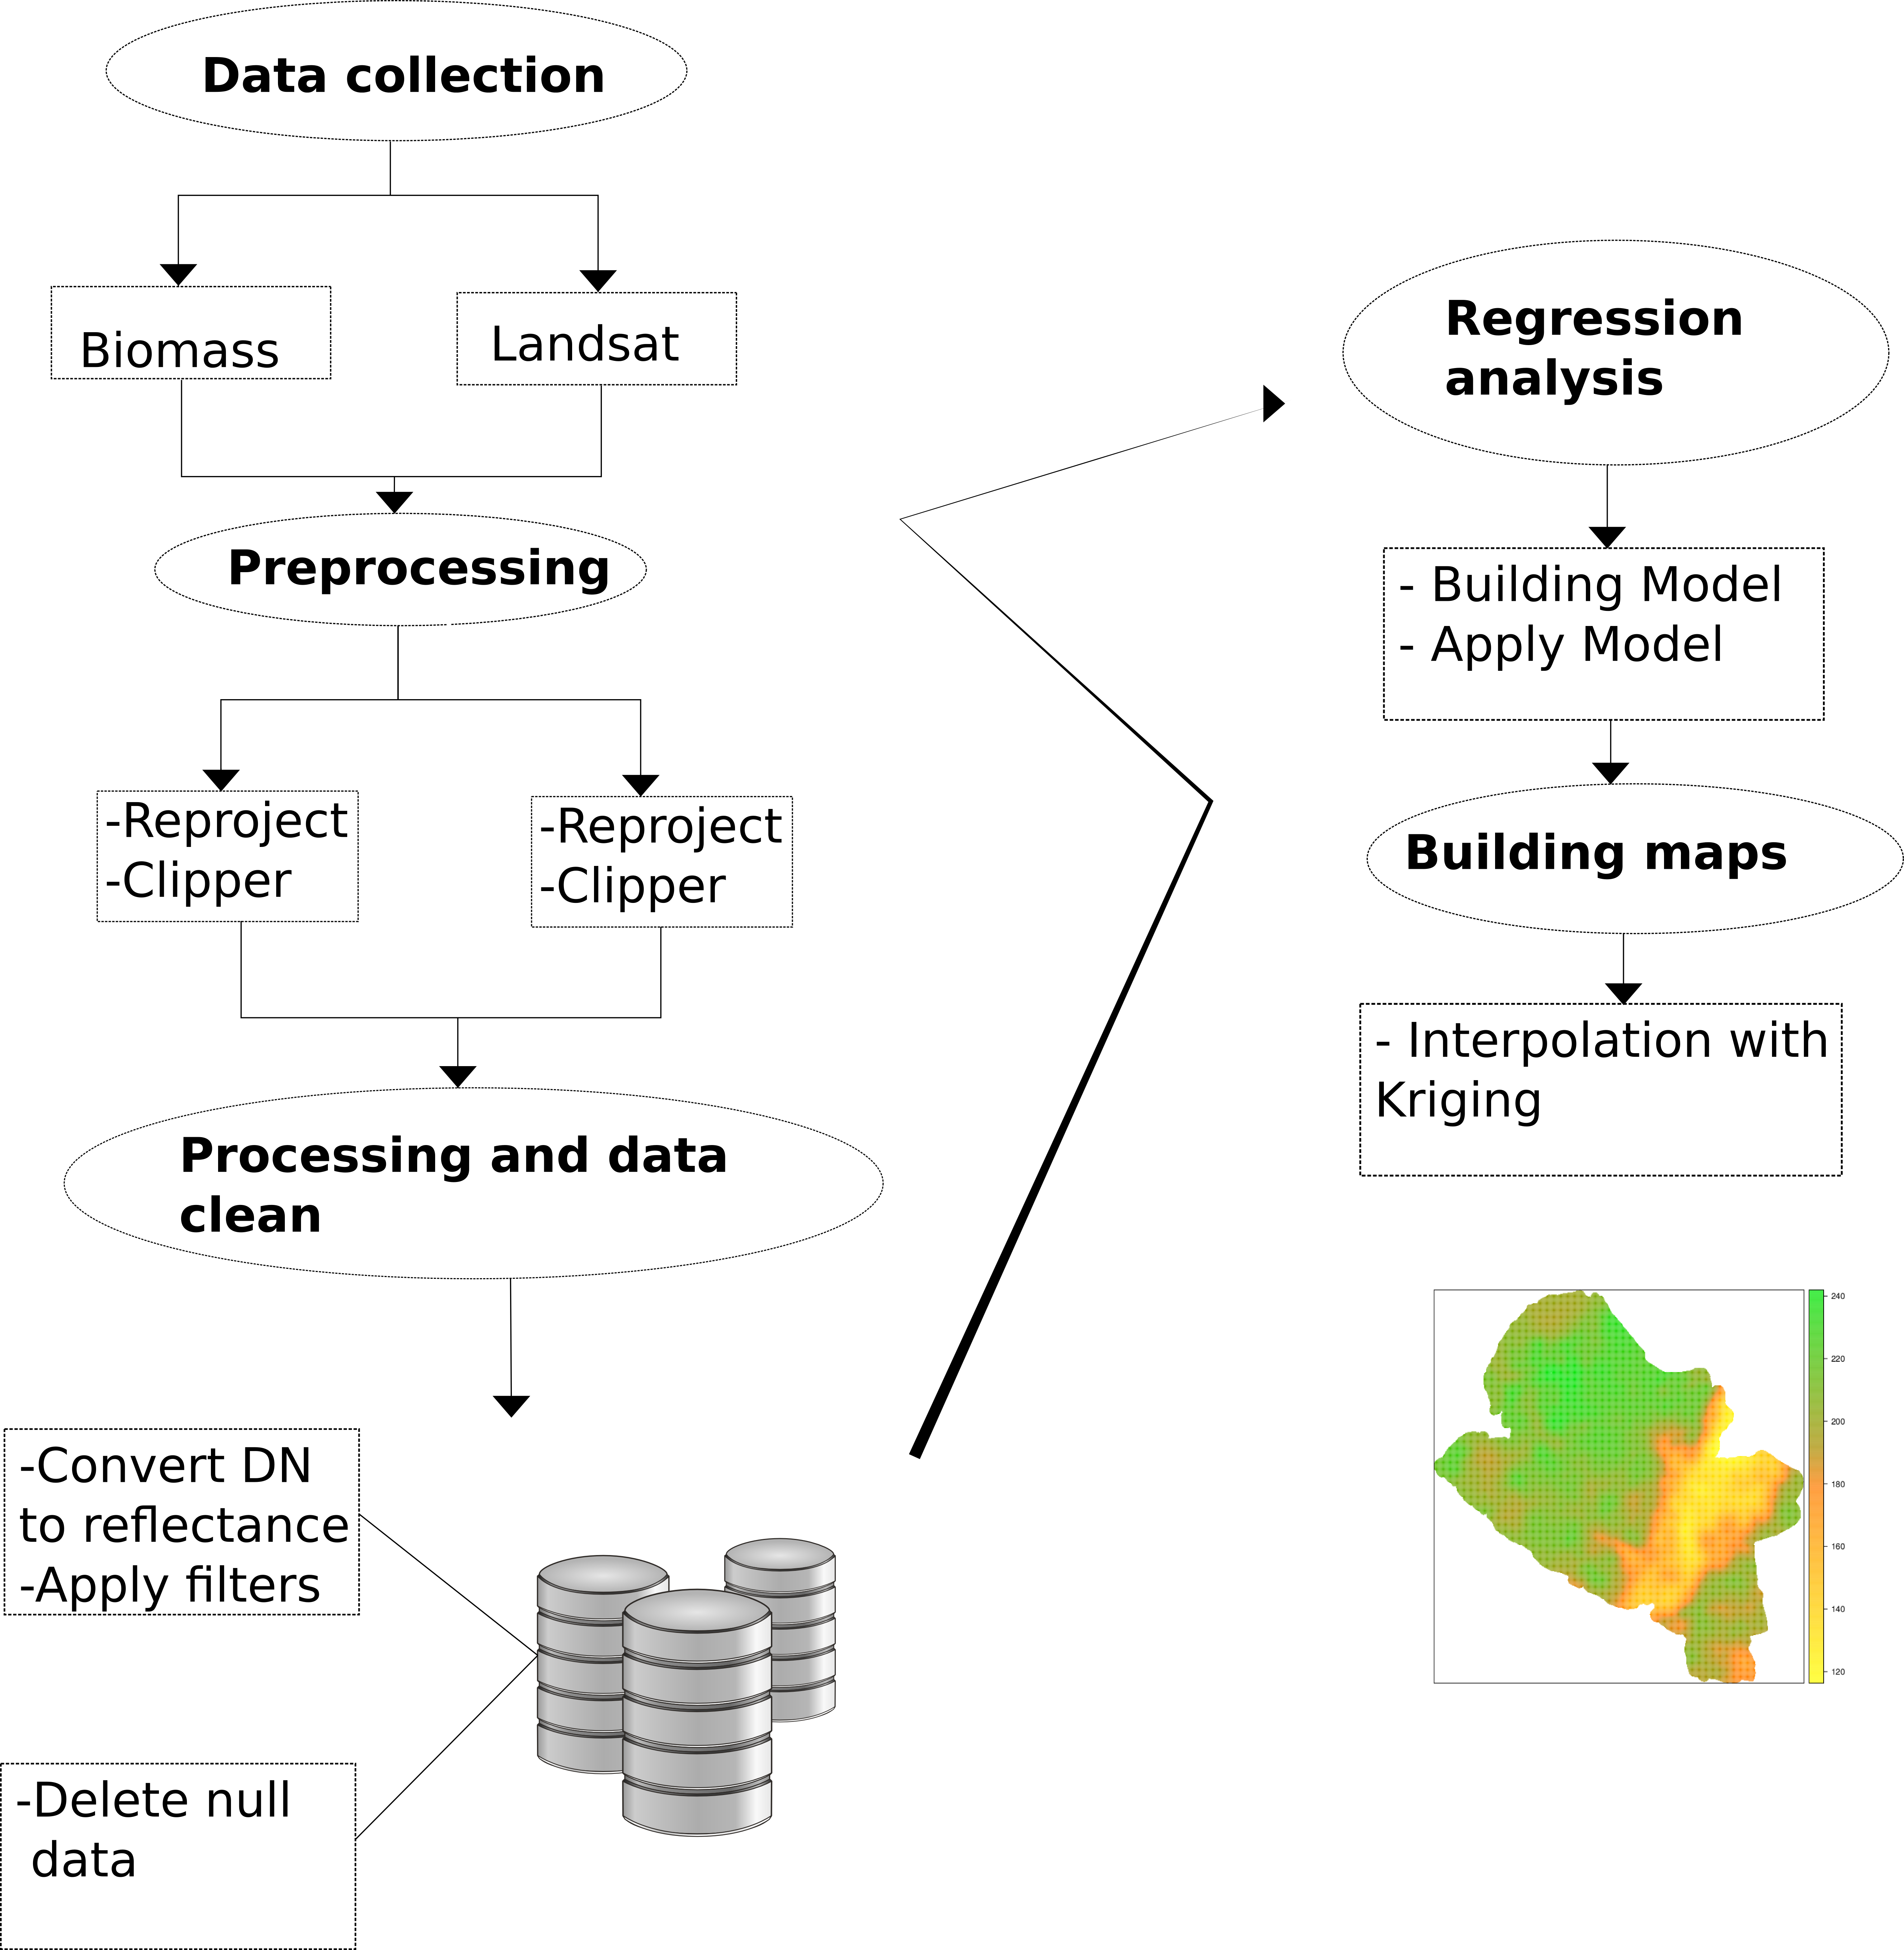
\includegraphics[width = 0.5\textwidth]{metodology.png}
  \caption{Metodología}
  \label{fig:metodology}
\end{figure}

\subsection{Obtención de datos}

El proceso de obtención de datos se realizó tomando imágenes satelitales proveidas por el sensor Landsat 7 ETM+. En este proceso se descargaron 1362 imágenes satelitales desde el año 1999 hasta mediados del año 2015. Para cubrir el departamento en su totalidad fue necesario descargar imágenes de cinco escenas diferentes.  La figura \ref{fig:cuts}a detalle los respectivos identificadores (Path ID y Row ID) y extensión de cada una de las escenas usadas.

Igualmente, durante esta etapa se tuvo acceso al mapa de biomasa construido por \cite{baccini2008afirst}.  Este es un mapa con resolución espacial de 1 $Km^2$ construido a partir de un modelo basado en imágenes MODIS recolectadas durante el año 2000 y 2003.

\subsection{Preprocesamiento}

En esta etapa se realizó un trabajo básico de procesamiento sobre las imágenes adquiridas.  Primero, dada la extensión del área de estudio, las escenas descargadas tenían diferentes sistemas de coordenadas (EPSG:32618 y EPSG:32617).  Por motivos de visualización se decidió unificar el sistema de coordenadas usando EPSG:3857, popular entre las herramientas de mapeo y desarrollo de aplicaciones web.  Muchas de las escenas cubrían una gran área del Océano Pacifico así como de otros departamentos de la región.  Se recorto las imágenes para contener solo los datos referentes al departamento de Nariño.  La figura \ref{fig:cuts}b ilustra el resultado final de esta etapa.

\begin{figure}
  \centering
  \subfigure[Imágenes Satélitales de Nariño]{\label{Imágenes Satélitales Nariño} 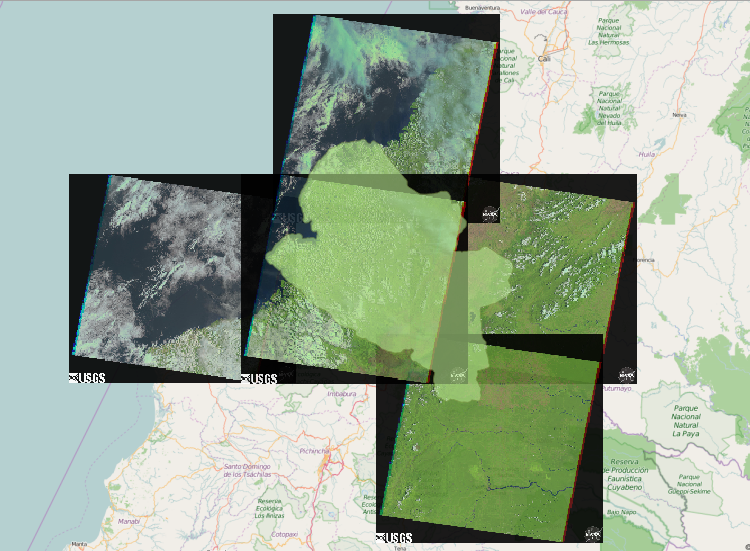
\includegraphics[width= 7cm]{cut1.png}}
  \vfill
  \subfigure[Imágenes recortadas de Nariño]{\label{Imágenes recortadas de Nariño}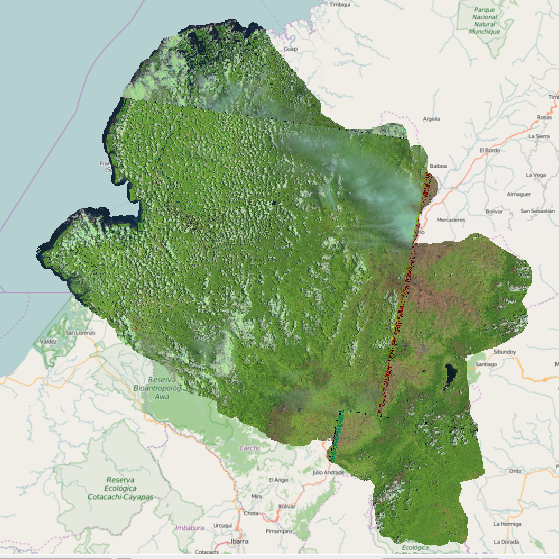
\includegraphics[width= 7cm]{cut2.png}}
  \caption{Prepocesamiento}
  \label{fig:cuts}
\end{figure}

De igual manera este proceso se lo realizó para el mapa de biomasa, como se muestra en la figura~\ref{fig:mapaNarino}

\begin{figure}
  \centering
  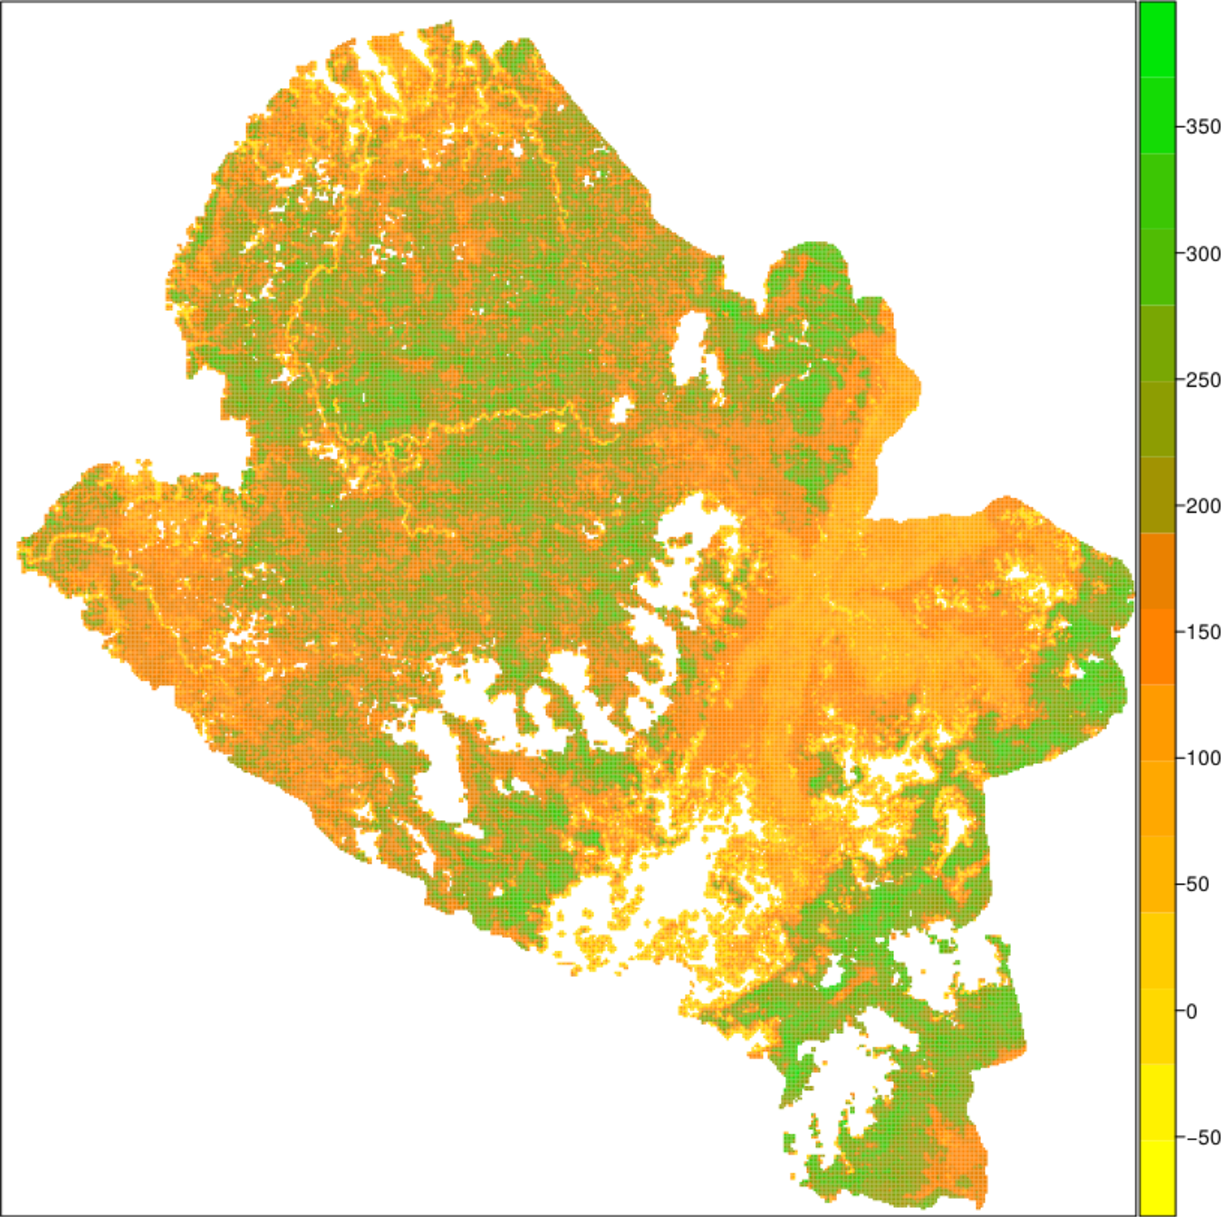
\includegraphics[width = 8cm]{mapaNarino.pdf}
  \caption{Mapa de biomasa en Nariño de 2000-2003 \cite{baccini2008afirst}}
  \label{fig:mapaNarino}
\end{figure}

\subsection{Procesamiento y limpieza de datos}

Se diseñó una base de datos para capturar los datos,
como lo muestra la figura~\ref{fig:landsatET}, la cual tiene 4 tablas. 

\begin{figure}
  \centering
  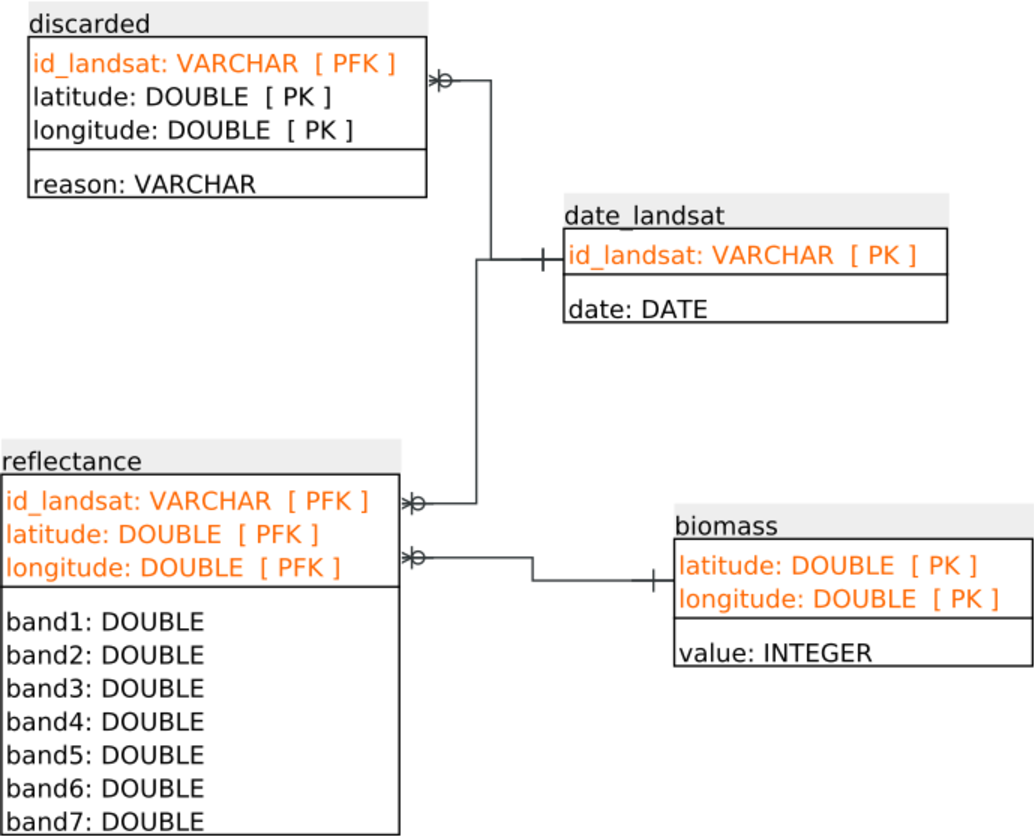
\includegraphics[width = 8cm]{landsatET.pdf}
  \caption{Modelo entidad-relacion Landsat}
  \label{fig:landsatET}
\end{figure}

Tabla date\_landsat: en la cual se almacenan las fechas de las imágenes satelitales.

Tabla reflectance: en la cual se almacenan los datos capturados y convertidos en reflentance,
de las bandas landsat (1 - 5,7) y la temperatura en grados kelvin de la banda 6.

Tabla discarded: en la cual se almacenan datos que fueron descartados, por varias razones,
son nubes calientes, nubes frias, datos ambiguos o no son vegetación.

Tabla biomass: en la cual se almacenan los datos de biomassa del mapa de \cite{baccini2008afirst}.

Para procesar las imágenes y llenar la base de datos se realizó un Script, el cual captura el Digital Number
de las imágenes satélitales y lo transforma en valor en reflectance. En este procesamiento de imagenes, se adiciono al Script unos filtros para para detección de nubes calientes,
nubes, frias, datos ambiguos como lo muestra el algoritmo propuesto por \cite{irish2000landsat}, además se aplico 
un filtro adicional, el NVDI(normalized difference vegetation index) para trabajar unicamente con datos de vegetación.

La tabla~\ref{tab:datos} muestra la relación de los datos obtenidos en este proceso.

\begin{table}
\caption{Datos obtenidos en en el proceso de procesamiento y limpieza  de datos}
\label{tab:datos}
\centering
\scalebox{0.7}{
\begin{tabular}{c c c}
\toprule
 Nombre & Valor& Detalle  \\
\midrule
Datos biomasa & 81.993 & Registros de biomasa para año 2000 a 2003 de  \cite{baccini2008afirst}\\
Datos biomasa usados & 140018 & Registros para construir el modelo grilla 450 metros\\
\hline
Imágenes landsat procesadas & 1321 & Imágenes de Nariño de 2000 a 2014 \\
Nube caliente & 3.731.768 & Registros de 2000 a 2014 \\
Nube Fria & 27.827.009 & Registros de 2000 a 2014 \\
No vegetacion & 3.459.210 & Registros de 2000 a 2014 \\
Ambiguo & 11.987.340 & Registros de 2000 a 2014 \\
\hline
Total Datos Descartados & 47.005.327 & Total datos descartados \\
Datos Validos Reflectance & 4.071.185 & Registros de 2000 a 2014 \\
\hline
Datos Totales & 51.076.512 & Registros Totales desde año 2000 a 2014 \\
\bottomrule
\end{tabular}}
\end{table}

\subsection{Análisis de regresión}

El análisis de regresión se realizó tomando los valores de las bandas landsat obtenidas año 2000 y 2003 y el valor de biomasa obtenido en \cite{baccini2008afirst},
para poder obtener un mejor modelo se agrupó y se saco un promedio con valores de las bandas landsat en cada punto, se fue iterando con  valores que superaban al menos N número de
muestras, siendo N desde 1 hasta 45 muestras, el mejor modelo obtenido fué cuando el número de muestas en cada punto superaba al menos las 35 muestras, este conjunto
de datos obtenido tenía 1009 registros. El comportamiento en las demás iteraciones muestra que con menos muestras hay más registros y eso hace que no se encuentre un buen modelo,
pero cuando hay mas muestras los registros son menores y esto también hace que el resultado del modelo tampoco sea bueno.

En la tabla~\ref{tab:metricas} se muestra las métricas de los modelos analizadas con 35 muestras y 1009 datos, el cual es el mejor modelo, esta tabla 
se la realizó usando la biblioteca de código abierto rminer presentada por \cite{cortez2010data} para la herramienta R.

\begin{table}
\caption{Métricas de modelos analizados con 35 muestras y 1009 datos}
\label{tab:metricas}
\centering
\scalebox{0.7}{
\begin{tabular}{c c c c c c c}
\toprule
 & SAE& MAE & RAE & RMSE & COR & R2 \\
\midrule
ctree & 10406.58225 & 30.88007 & 65.04650 & 40.02893 & 0.69401 & 0.48165 \\
rpart & 10197.95826 & 30.26100 & 63.74249 & 39.37592 & 0.70520 & 0.49730 \\
kknn & 9147.51425 & 27.14396 & 57.17667 & 36.86581 & 0.74955 & 0.56182 \\
mlp & 9179.79310 & 27.23974 & 57.37843 & 34.70711 & 0.78122 & 0.61031 \\
mlpe & 8746.27740 & 25.95335 & 54.66874 & 34.57953 & 0.78309 & 0.61323 \\
ksvm & \textbf{8462.61487} & \textbf{25.11162} & \textbf{52.89570} & 34.67742 & \textbf{0.79830} & \textbf{0.63729} \\
randomForest & 8807.76477 & 26.13580 & 55.05306 & 34.70615 & 0.78239 & 0.61214 \\
mr & 10410.13919 & 30.89062 & 65.06873 & 38.61068 & 0.72000 & 0.51840 \\
mars & 8842.91866 & 26.24011 & 55.27279 & \textbf{33.96852} & 0.79161 & 0.62665 \\
cubist & 9012.54150 & 26.74345 & 56.33302 & 35.70576 & 0.77611 & 0.60235 \\
pcr & 10337.63121 & 30.67546 & 64.61552 & 38.59290 & 0.72023 & 0.51873 \\
plsr & 10337.63121 & 30.67546 & 64.61552 & 38.59290 & 0.72023 & 0.51873 \\
cppls & 10337.63121 & 30.67546 & 64.61552 & 38.59290 & 0.72023 & 0.51873 \\
\bottomrule
\end{tabular}}
\end{table}

En este proceso tambien se usó el paquete R Boruta \cite{kursa2010feature}, el cual es un nuevo algoritmo de selección de características 
para encontrar todas las variables relevantes. El algoritmo está diseñado como un recubrimiento alrededor 
del algoritmo de clasificación random forest. Esto para saber si todas las bandas de landsat utilizadas eran relevantes para encontrar biomasa, 
en la figura~\ref{fig:boruta} se puede observar la relevancia de las bandas landsat para encontrar biomasa en el mejor modelo.

\begin{figure}
  \centering
  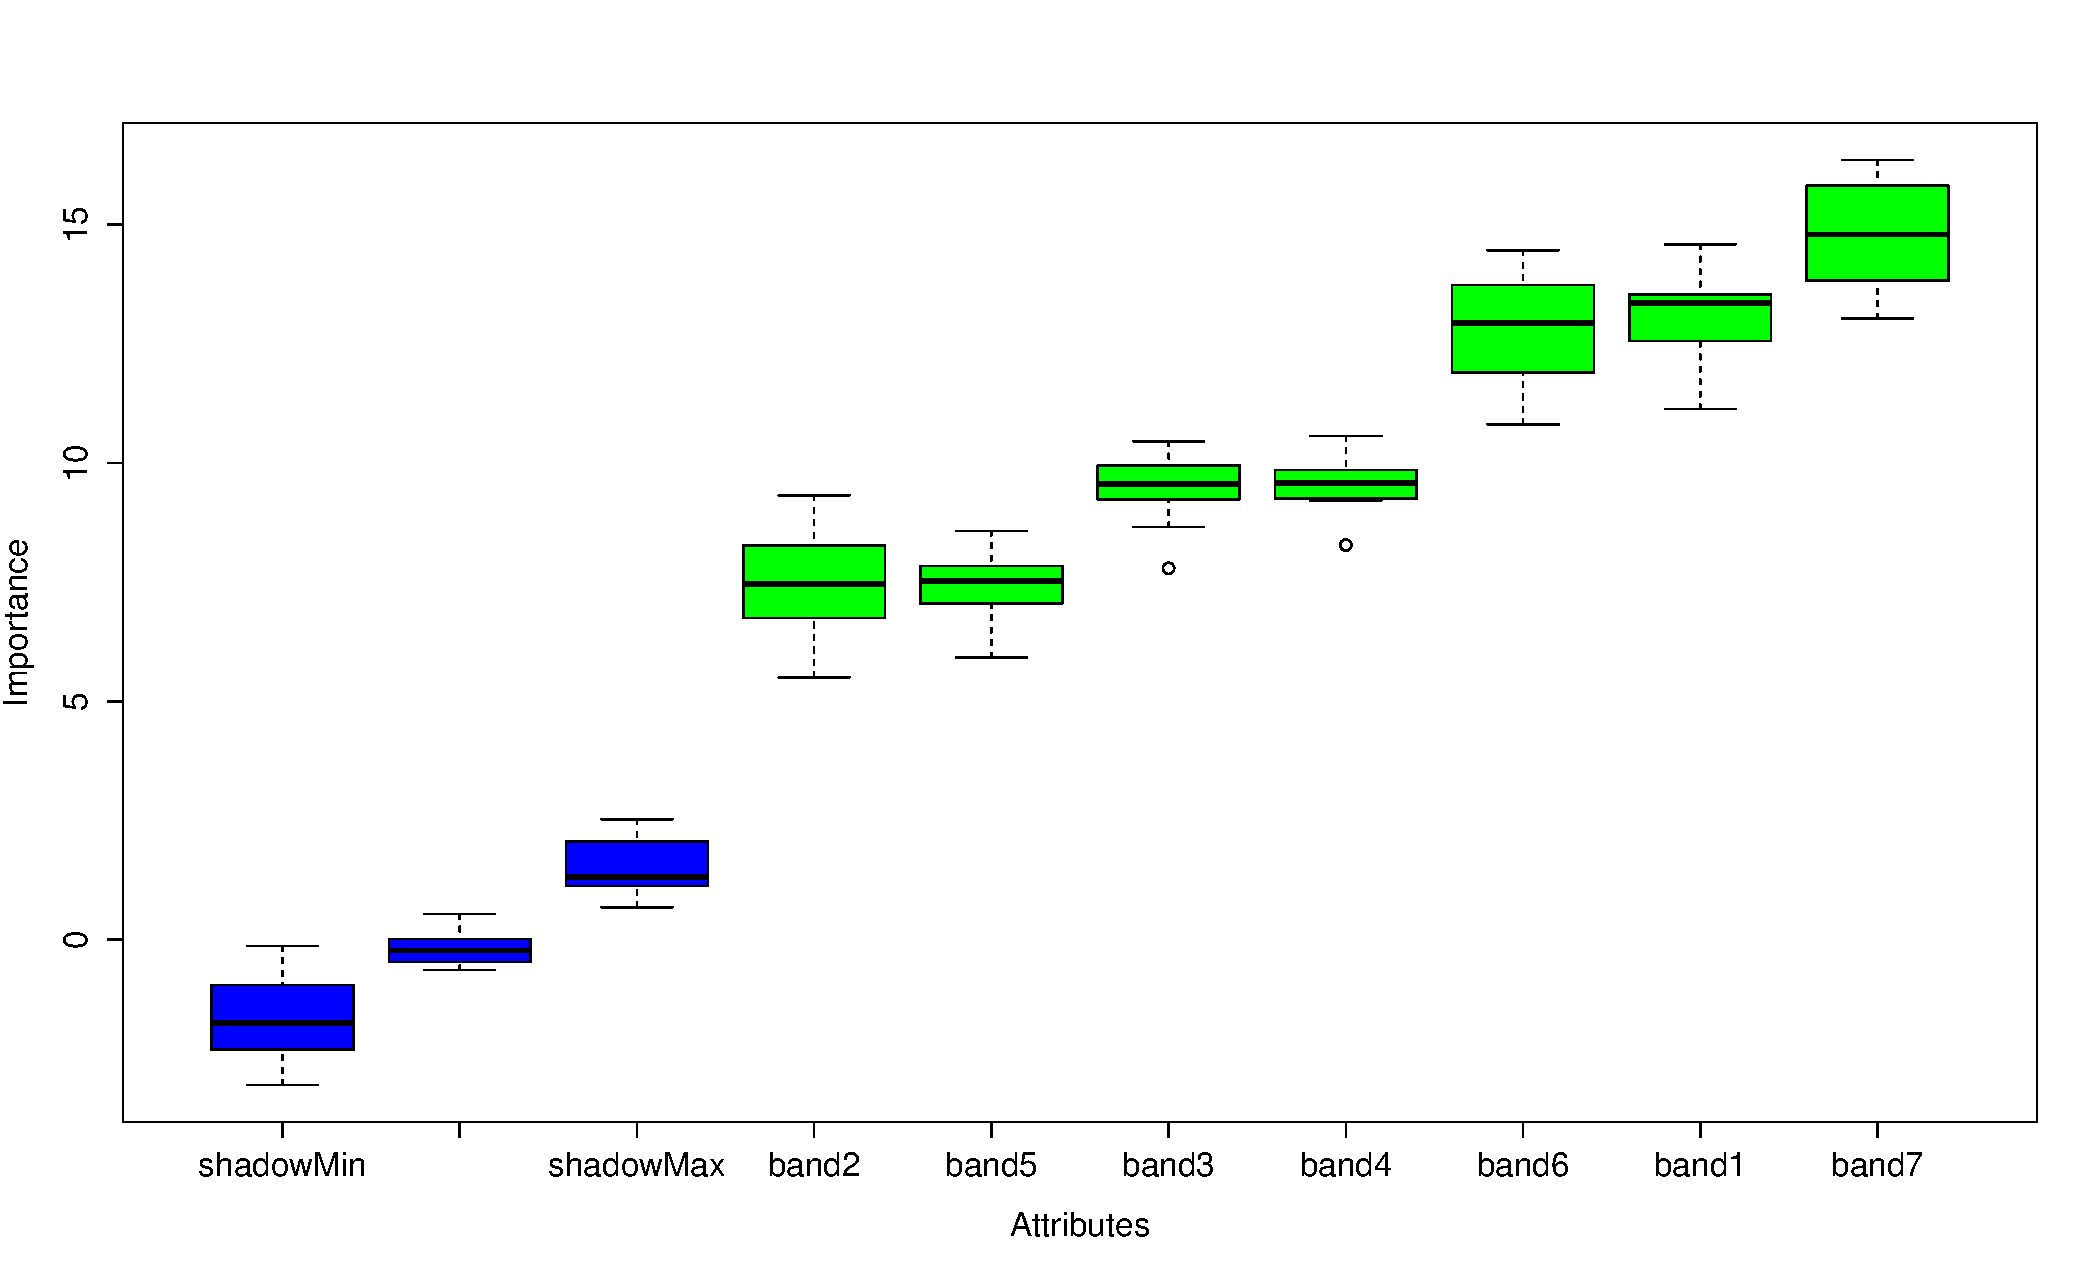
\includegraphics[width = 8cm]{boruta.pdf}
  \caption{Relevancia de bandas landsat en el análisis de regresión}
  \label{fig:boruta}
\end{figure}

\subsection{Construcción de mapas}

Para la construcción de mapas de biomasa se utilizó el método Kriging que provee una solución al problema 
de la estimación basada en un modelo continuo de variación espacial estocástica, el objetivo de Kriging es el de estimar el valor de una 
variable aleatoria, Z, en uno o más puntos no muestreados o sobre grandes bloques. 

El método Kriging recibe como entrada datos de la muestra, y una malla dependiendo de la resolución que se quiera obtener, por ello los datos de muestra se
obtuvieron aplicando el modelo obtenido en el análisis de regresión a datos agrupados en cada punto por mes, año y uno general entre el año 2000 a 2014; y la 
 malla se construyó con puntos regulares espaciados cada 450 metros. 
 
 En la figura~\ref{fig:biomasaMes}, figura~\ref{fig:biomasaAnio}, figura~\ref{fig:biomasaTotal}  se muestra los mapas obtenidos por meses, años y general entre el año 2000 a 2014 respectivamente. 
 
\begin{figure}
  \centering
  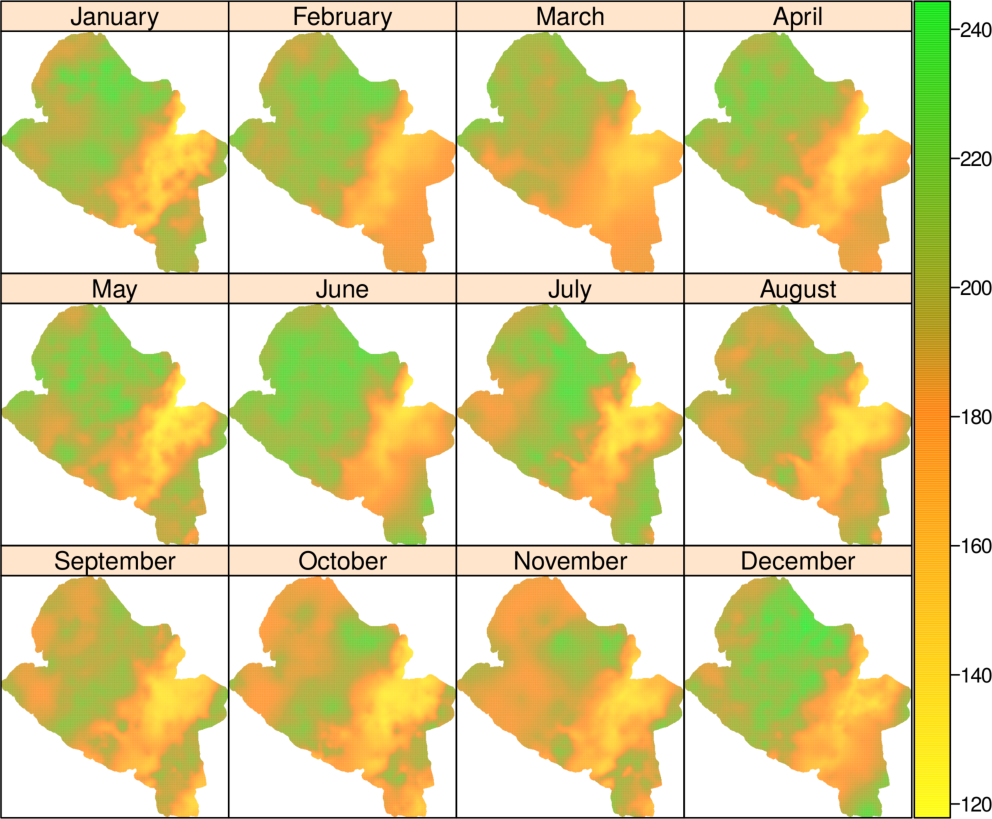
\includegraphics[width = 8cm]{mapMonthsBiomass.pdf}
  \caption{Mapas biomasa por meses}
  \label{fig:biomasaMes}
\end{figure}

\begin{figure}
  \centering
  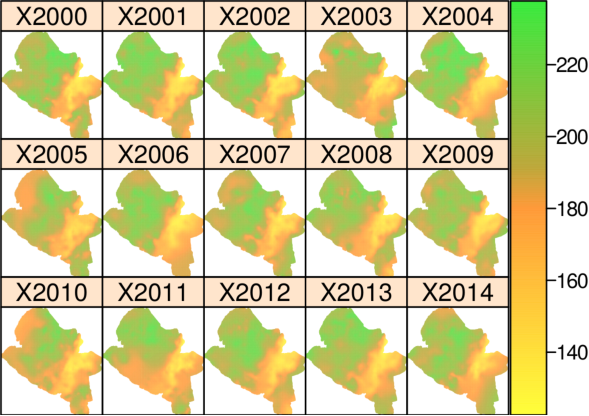
\includegraphics[width = 8cm]{mapYearsBiomass.pdf}
  \caption{Mapas biomasa por años}
  \label{fig:biomasaAnio}
\end{figure}

\begin{figure}
  \centering
  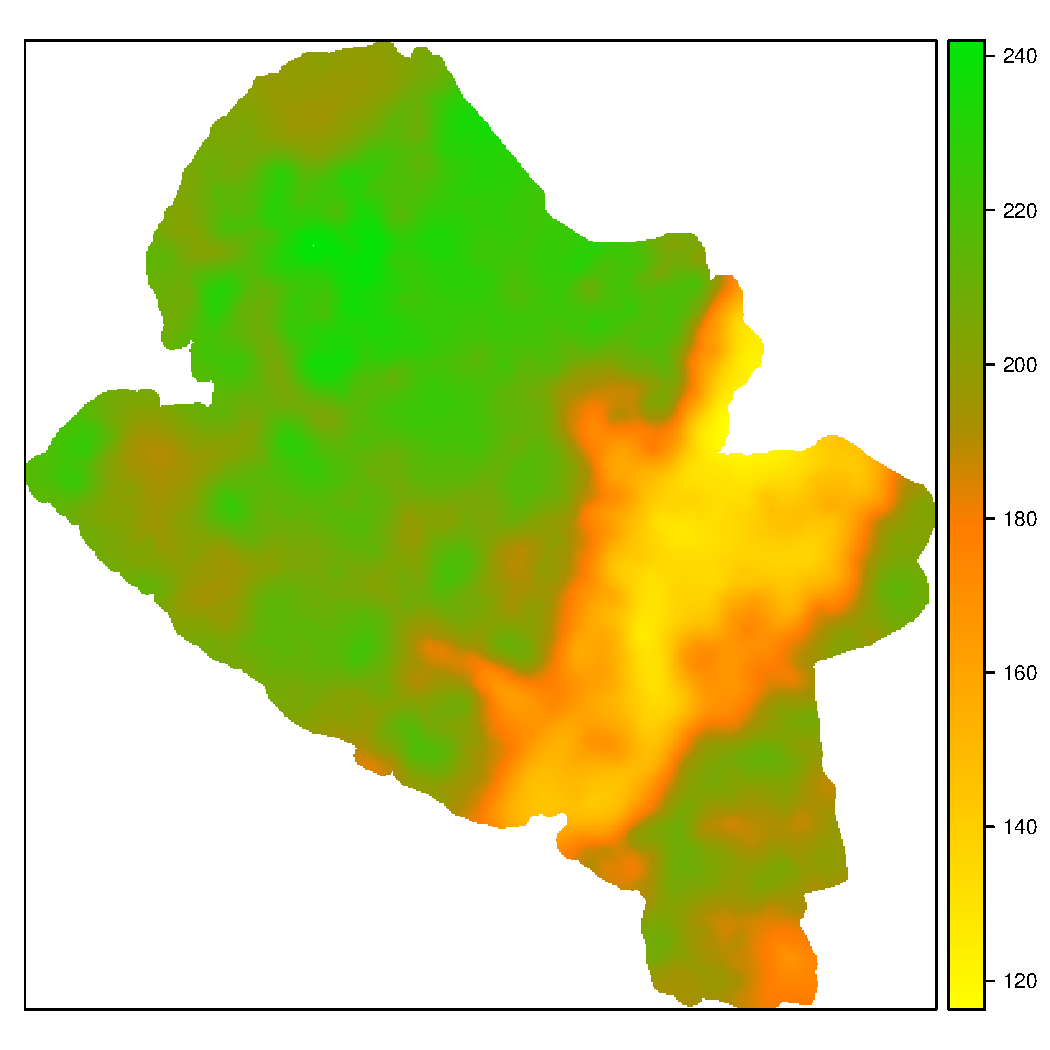
\includegraphics[width = 8cm]{mapGeneralBiomass.pdf}
  \caption{Mapas biomasa general años 2000-2014}
  \label{fig:biomasaTotal}
\end{figure}

%\section{Conclusiones}

Se construyeron mapas energéticos con el componente solar en el departamento de Nariño,
usando los sensores Landsat 7 y MODIS.

Las imágenes sateliatles son una gran fuente de información debido a la capacidad de almacenar gran cantidad de registros históricos para diferentes tipos de datos, estos datos
poco a poco estan siendo utilizados por organizaciones para determinar características terrestres, fenómenos naturales, condiciones de los mares,
características de la vegetación, etc. Por esta razón el uso de imágenes satelitales
en la investigación da resultados aproximados y a bajo costo, teniendo en cuenta el costo
que puede implicar hacer muestreo en campo.

Se construyo una metodología para la construcción de mapas energéticos con el potencial
de radiación solar, el cual se lo puede aplicar en zonas donde no tengan estaciones climáticas con los sensores Landsat o MODIS.

En la construcción del mejor modelo, con ambos sensores Landsat 7 y MODIS se tubo un $R^2$ por encima del 90\%,
teniendo en cuenta que las imágenes landsat 7 se obtienen cada 16 dias y las de MODIS son diarias, sería
de mayor provecho usar el sensor MODIS para hacer estudios posteriores con series de tiempo.

Tanto la correlación como el $R^2$ entre los mapas construidos a partir del sensonr Landsat 7 y MODIS
es buena, teniendo en cuenta que en el mapa general se tiene una correlación del 94\% y un $R^2$ del
88\%.



%\appendices
%\section{Repositorio}
%El código fuente y conjunto de datos se encuentran en el repositorio de github.


\ifCLASSOPTIONcompsoc
  % The Computer Society usually uses the plural form
  \section*{Agradecimientos}
\else
  % regular IEEE prefers the singular form
  \section*{Agradecimientos}
\fi

Esta investigación se hizo posible gracias a los recursos otorgados por el Sistemas General de Regalias en el marco de proyecto ``Análisis de Oportunidades Energéticas con Fuentes Alternativas en el Departamento de Nariño'' ejecutado por el programa de Ingeniería Electrónica de la Universidad de Nariño.

% Can use something like this to put references on a page
% by themselves when using endfloat and the captionsoff option.
\ifCLASSOPTIONcaptionsoff
  \newpage
\fi


\bibliographystyle{plain}
\bibliography{bibliography}

\end{document}
